\documentclass[11pt,a4paper]{article}
\usepackage[utf8]{inputenc}
\usepackage[english]{babel}
\usepackage{amsmath}
\usepackage{amsfonts}
\usepackage{amssymb}
\usepackage{graphicx}
\usepackage[left=1.4cm,right=1.4cm,top=0.7cm,bottom=1.8cm]{geometry}
\usepackage{footnotebackref}
\usepackage{hyperref}
\hypersetup{
    colorlinks=true,
    linkcolor=blue,
    urlcolor=blue}
\author{Vernay Amélie}
\title{%
    \begin{minipage}\linewidth
        \centering
        HMMA238 - Individual challenge
        \vskip3pt
        \large Methodology for the prediction part
    \end{minipage}
}


\begin{document}
\maketitle

Before diving into my methodology, here are the links to my different works:
\begin{itemize}
\item \href{https://github.com/AmelieVernay/Pred_Bike_Challenge}{GitHub repository for the prediction part}
\item \href{https://github.com/AmelieVernay/MtpBikeViz}{GitHub repository for the visualization part}
\item \href{https://amelievernay.pythonanywhere.com/}{Direct link to my visualization work}
\end{itemize}

\section*{Goal}

The goal of the prediction part of this challenge is to predict the number of bicycle passing between 00:01 AM and 09:00 AM on Friday, April 2nd 2021 on the bike counting totem located on \textit{Place Albert 1er, Montpellier}.

\section*{Main ideas}

\begin{itemize}
\item The bike traffic this time last year does not seem like a relevant indicator to me. Indeed, on 16 March 2020, a lockdown was announced to fight the Covid-19 pandemic in France...remember ? So cycle paths were kind of...calm.
\item When it comes to choosing a means of transport for daily commuting, \textbf{weather} is a key criterion.
\item The time period aimed by this prediction is the \textbf{morning of a working day}. I really think that this point should be taken into account.
\end{itemize}

\section*{My approach}

To deal with the weather aspect, I chose to "build" my own dataset throughout the month of March. I believe that sometimes, the actual \textit{felt} weather is far away from public weather reports, plus, as an every day cyclist, I think that some conditions are more likely to dissuade one from taking its bike than others. So I wrote a \texttt{python} function that updates a dataset everyday with the given input values for rain, wind, and nebulosity. As spring is coming, I chose not to include temperature. The underlying idea was to use the dataset to predict bike traffic using linear regression. \textbf{Problem:} it didn't rained ! And as I would have expected, wind and nebulosity are clearly not good explanatory variables in that case... My model isn't justified.\\

I then thought about times series forecasting, but I didn't wanted to use programming tools that I don't fully understand mathematically.\\

I decided to keep things simple. The dataset we were given was kind of messy. The concept of an open contribution for collecting data is beautiful, but the result is like a Swiss cheese: full of holes. Indeed, sometimes there is no entry until 10 PM where suddenly 1304 people pass on the totem. The next day we have 11 entries every 2 minutes around 7 AM and that's it\footnote{The first thing I thought about was to actually contribute, when I have time to do so. I sometimes pass near by the totem and I discovered I could enter data myself \href{https://docs.google.com/forms/d/e/1FAIpQLSfPHrWpHSj0A0VHzkaBlvSYCgUBQQyQOPOJ6lhq0dIDLvcDlg/viewform}{here}. But this is not great step forward...}.
So I wrote a bunch of \texttt{python} functions to deal this dataset. The most important ones are probably \texttt{drop\_hour\_gap} and \texttt{resamp\_interp}. The first one drops the days for which we don't have a first entry before a given hour. For example, using it with \texttt{hour=12} would keep only the days of the given dataframe for which there is at least one entry before 12 AM. The motivation for this function is to initialize a "correct" dataset to give to the next function \texttt{resamp\_interp}. This one downsamples the dataset to the greatest common time basis: minute, sets zero values for the time 00:00 to 00:59 on each day\footnote{It could have been only for 00:00 but since almost no bike are passing on the totem at this time of the day, well I found it more relevant to set this to zero for the coming interpolation purpose.}, and interpolates the values to fill the \texttt{NaN} values appeared when resampling. I applied these (and others) functions on the extracted data for the month of March, in the notebook \texttt{resamp\_interp\_test.ipynb} to check visually the relevance of my method. The result looks like this:\\

\begin{center}
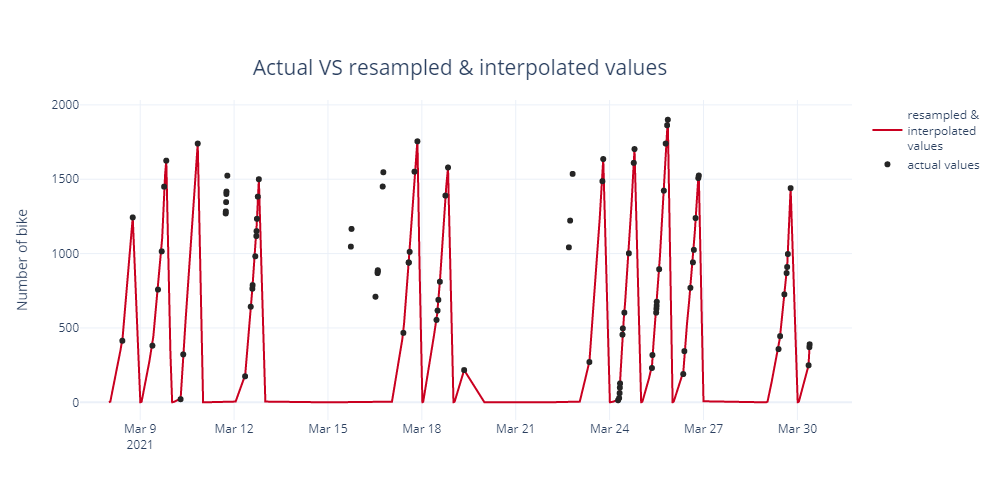
\includegraphics[scale=0.35]{resamp_interp.png}
\end{center}


Lonely floatting dark points correspond to values for days where the first data collected occured after 12 AM, so for the same axis, the points corresponding in the interpolated dataset were set to zero by the \texttt{drop\_hour\_gap} function. This is why the red line lies on the $x$-axis: it was too risky to use these points for interpolation. We can see that the remaining points are related by the red line in a pretty intuitive way. This\footnote{and a close look at the two dataframes,} let's me think that the method is ok. I now have a filled dataframe with coherent values for each minute of each day. I can just grab those corresponding to 9 AM!\\

With this pre-process on the data, I then chose to simply analyse the behaviour of bike traffic on these past months. I did this in notebook \texttt{forecast.ipynb}. Looking only at the values at 9:00 AM, I tried to answer the following questions: "Is the traffic increasing with the arrival of "good weather days" ?", "Is the traffic the same on each day of the week ?", "Does the recent time change seem to have affected bike traffic ?"...\\

After some investigations, I noticed that, only considering data from the beginning of March, on week days, at 9:00 AM, the mean from the beginning of the month, to any following day was \textit{almost} constant. I extracted a dataframe whose first row contained the mean of the values from the beginning of March up to today, whose second row contained the mean of the values from the beginning of March up to yesterday, whose third row contained the mean of the values from the beginning of March up to the day before yesterday, whose fourth row contained...well we got it. All of the values lie around $325$, and for the first five rows, we have, from oldest to most recent, $327.5$, $328.0$, $328.2$, $329.7$, $334$. I think it could be reasonable to consider that the next value, i.e. the mean of the values from the beginning of March up to tomorrow, shouldn't be too far away from\footnote{yes the cumulative means are increasing, but today's value was particularly high, and friday values are always a bit under thursday ones} $333$.

For this to be true, I simply needed to solve a single-unknown equation. Namely, if $m = 333$, $x =$"tomorrow's value", $l$ is the lenght of tomorrow's dataframe-for-this-month-values, and $S$ is the sum of all the values in today's dataframe-for-this-month-values then,
$$
\frac{(S + x)}{l} = m\ \Longleftrightarrow\ x = (m \times l) - S
$$

I know $m$ and I can easily compute $S$ and $l$. This, rounded to the nearest integer, gives me $x = 316$. And because I plan on going to the farmers market tomorrow morning\footnote{and not because I prefer odd numbers...}, I am going to add $1$ to this prediction. That's it, my prediction number is $317$, and I can't wait until tomorrow to see how far I am from the actual value!

\end{document}